\subsection{システム}
\label{tag:function}
本研究では、プラグインとしてLMS上に新しい機能を提供するのではなく、LTIに準拠したWebアプリケーションを用いて、異なるLMSで同様の機能が提供でき、Webアプリケーション側での操作に対しLMS側に特定の点数を返すことを目的とした。そこで、異なる仮想マシン上にそれぞれLMSであるCanvas、Moodleと、独立したWebアプリケーションとしてネットワーク自己学習機能を導入した。また、ネットワーク自己学習機能はRuby on Railsを用いて実装した。これらは図\ref{fig:virtualMachine}で表しているようにネットワーク自己学習機能は実際には独立したWebアプリケーションであるが、あたかもLMS側にプラグインとして導入されているように機能を提供する。

\begin{figure}[htbp]
  \begin{center}
    \resizebox{\textwidth}{!}{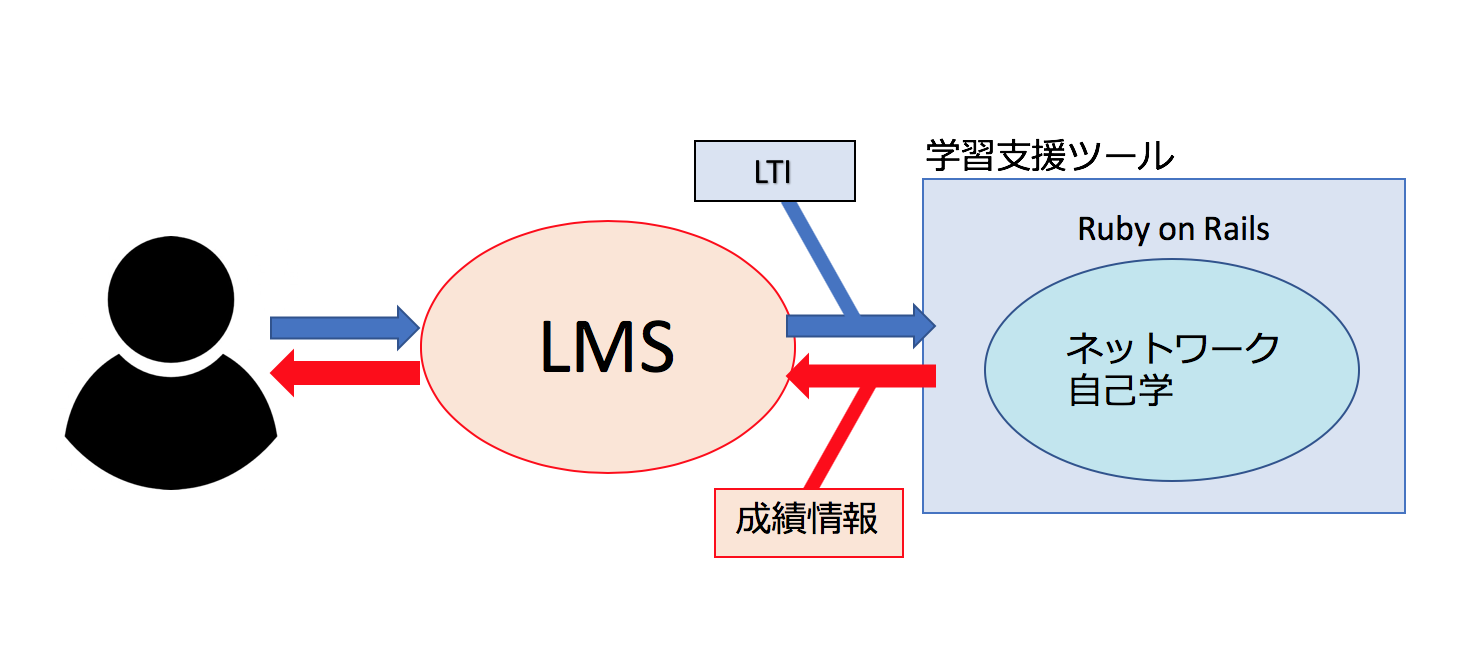
\includegraphics{img/system.png}}
    \caption{本研究で提案するシステムの構成}
    \label{fig:virtualMachine}
  \end{center}
\end{figure}



また、Webアプリケーション側はLMSに呼び出された際、独立したWebアプリケーションとしてネットワーク自己学習機能を提供する。この機能にはネットワークを自由に構成し、機器情報を設定することのできる自由描画モードと、予め問題として構成されたネットワークに正しい機器情報を追加することで正しいネットワークの作成を目指す問題演習モードが有る。問題演習モードでの正誤によって得られた得点をLMS側に返すことでLMSでの学習者の評価を行う。\\
魚本ら[1]の制作したネットワーク自己学習機能はMoodleの独自プラグインとしてネットワーク自己学習機能を実装している。
クライアントサイドである独自プラグインとしてのシミュレータ部分はHTMLとJavaScriptで、Moodleのプラグインとしての設定の部分はPHPで、シミュレータで作成されたネットワークの構成の正誤の判定プログラムはRubyでそれぞれ記述されている。これは、様々なシステムを使用しているため、複数のシステム間でデータのなどの連携を行わなければならず、安定性にかけていた。\\
 そこで、本研究ではすべてのシステムをRuby on Railsの中で実装した。MVCアーキテクチャに基づいて設計することにより、魚本[1]らのシステムをすべてRuby on Rails内で実現した。これにより、複数のシステム間でのデータの送受信などを行う必要性がなくなり、システムとしての安定性を実現した。
